% =============================================================================
\chapter{Análise exploratória de dados}\label{cap:eda}
% =============================================================================

A análise exploratória foi feita sobre a base tratada e validada. Todos os
gráficos deste capítulo foram gerados no notebook do \textit{Checkpoint}~2 e
seguem as mesmas convenções visuais, descritas no \autoref{cap:storytelling}:
o título de cada gráfico enuncia a conclusão, e as cores têm função fixa
(azul para compra ou série principal, laranja para venda, cinza para contexto).

\section{Estatística descritiva dos negócios}\label{sec:descritiva}

\begin{table}[htbp]
\caption{\label{tab:descritiva}Estatística descritiva de preço, quantidade e valor dos negócios}
\begin{corpotabela}
\begin{tabular}{lrrr}
\toprule
Estatística & Preço (USDT) & Quantidade (BTC) & Valor (\usd) \\
\midrule
Contagem & 27.925.338 & 27.925.338 & 27.925.338 \\
Média & 93.590,88 & 0,00708 & 661,06 \\
Desvio-padrão & 3.823,32 & 0,05673 & 5.308,24 \\
Mínimo & 86.050,99 & 0,00001 & 0,86 \\
1.º quartil & 89.376,53 & 0,00006 & 5,65 \\
Mediana & 95.256,31 & 0,00006 & 5,87 \\
3.º quartil & 96.469,59 & 0,00029 & 26,93 \\
Percentil 99 & 99.160,55 & 0,15022 & 13.940,28 \\
Máximo & 99.475,00 & 56,34875 & 5.433.099,71 \\
Assimetria & $-0,47$ & 92,77 & 95,33 \\
Curtose em excesso & $-1,21$ & 49.183,05 & 53.063,31 \\
Coeficiente de variação & 0,04 & 8,01 & 8,03 \\
\bottomrule
\end{tabular}
\end{corpotabela}
\fontedados
\end{table}

A \autoref{tab:descritiva} mostra dois comportamentos opostos. O preço oscilou
entre \usd~86 mil e \usd~99,5 mil, com coeficiente de variação de apenas 4\,\%,
mas sua distribuição é bimodal (antes e depois da queda), e a média sozinha
engana. Já o valor dos negócios tem mediana de \usd~5,87 e média de
\usd~661,06: a média é mais de cem vezes a mediana, com assimetria de 95 e
curtose de 53 mil. Para descrever o negócio típico, só a mediana faz sentido.
A \autoref{fig:hist} confirma que a maior parte dos negócios é minúscula.

\begin{figure}[htbp]
\caption{\label{fig:hist}Distribuição do valor dos negócios em escala logarítmica}
\begin{center}
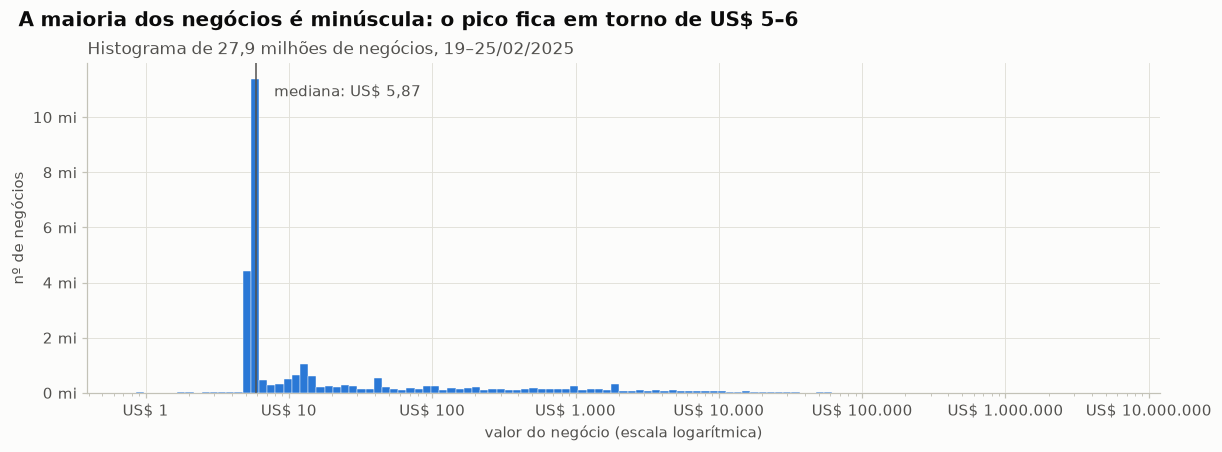
\includegraphics[width=\textwidth]{figuras/fig_hist_tamanho.png}
\end{center}
\fontedados
\end{figure}

\section{Concentração do volume por faixa de tamanho}\label{sec:faixas}

O agrupamento por faixa de tamanho (\code{groupby} em \code{size_bucket})
responde à segunda parte da pergunta P2: quem concentra o volume?

\begin{table}[htbp]
\caption{\label{tab:faixas}Negócios e volume financeiro por faixa de tamanho}
\begin{corpotabela}
\begin{tabularx}{\textwidth}{L{3.0cm}RRRRR}
\toprule
Faixa de tamanho & Negócios & Volume (\usd~mi) & Ticket mediano (\usd) & \% dos negócios & \% do volume \\
\midrule
$<$ \usd~100 & 23.123.213 & 276,70 & 5,78 & 82,80 & 1,50 \\
\usd~100 a 1 mil & 2.533.123 & 1.029,09 & 304,45 & 9,07 & 5,57 \\
\usd~1 mil a 10 mil & 1.871.733 & 6.118,64 & 2.134,25 & 6,70 & 33,14 \\
\usd~10 mil a 100 mil & 387.566 & 9.436,34 & 17.067,95 & 1,39 & 51,12 \\
$\geq$ \usd~100 mil & 9.703 & 1.599,66 & 120.057,53 & 0,03 & 8,67 \\
\midrule
Total & 27.925.338 & 18.460,44 & 5,87 & 100,00 & 100,00 \\
\bottomrule
\end{tabularx}
\end{corpotabela}
\fontedados
\end{table}

\begin{figure}[htbp]
\caption{\label{fig:faixas}Participação de cada faixa na contagem e no valor dos negócios}
\begin{center}
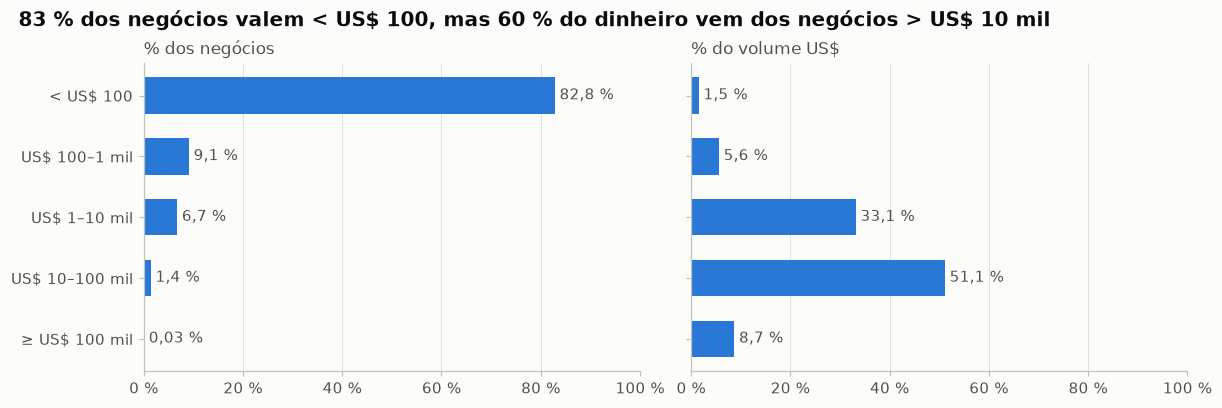
\includegraphics[width=\textwidth]{figuras/fig_faixas_tamanho.png}
\end{center}
\fontedados
\end{figure}

A \autoref{tab:faixas} e a \autoref{fig:faixas} mostram uma \textbf{concentração
extrema}: negócios abaixo de \usd~100 são 82,8\,\% da contagem e apenas 1,5\,\%
do valor, enquanto negócios a partir de \usd~10 mil são apenas 1,42\,\% da
contagem e respondem por 59,8\,\% do valor negociado. Para a mesa de execução,
contar negócios mede a atividade de robôs, e somar o valor financeiro mede a
liquidez de fato. As duas métricas contam histórias diferentes e precisam ser
vistas juntas.

\section{A semana em uma imagem}\label{sec:semana}

A \autoref{fig:precovolume} resume a semana: o preço subiu até o topo de
\usd~99.475 em 21/02, caiu com o ataque à Bybit, estabilizou no fim de semana e
desabou em 24 e 25/02, até o fundo de \usd~86.051. O volume por hora acompanha
os episódios de queda.

\begin{figure}[htbp]
\caption{\label{fig:precovolume}Preço de fechamento por minuto e volume por hora, de 19 a 25/02/2025}
\begin{center}
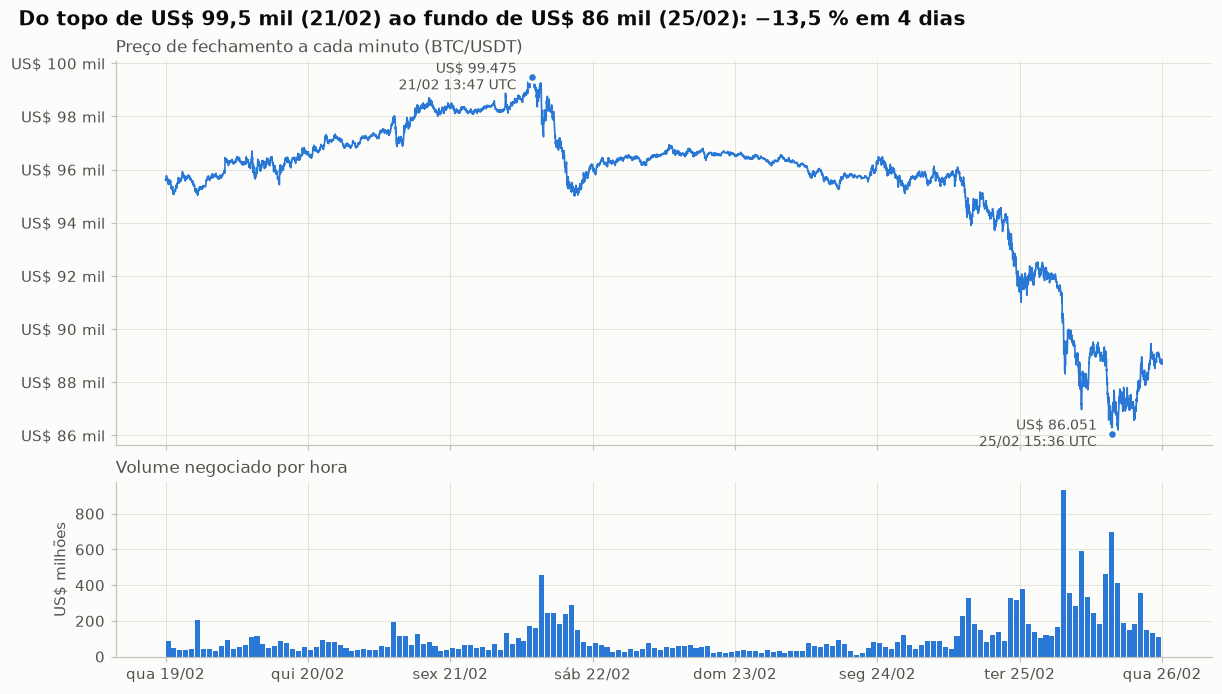
\includegraphics[width=\textwidth]{figuras/fig_preco_volume.png}
\end{center}
\fontedados
\end{figure}

\section{Resumo diário e dias de estresse}\label{sec:diario}

Para evitar a escolha subjetiva dos dias, cada dia foi classificado por uma
\textbf{regra objetiva}: amplitude intradiária
($\text{máxima}/\text{mínima} - 1$) acima de 4\,\% caracteriza um dia de
\textbf{estresse}; os demais são separados em dia útil e fim de semana, porque
no fim de semana o mercado é naturalmente mais calmo. A \autoref{tab:diario}
apresenta o resumo diário; a volatilidade realizada segue a
\autoref{eq:volrealizada}, e o saldo de fluxo é o OFI do dia em percentual.

\begin{table}[htbp]
\caption{\label{tab:diario}Resumo diário da semana e classificação dos dias}
\begin{corpotabela}
\setlength{\tabcolsep}{3.5pt}
\begin{tabular}{L{1.35cm}P{1.55cm}P{1.65cm}P{1.25cm}P{1.45cm}P{0.85cm}P{1.35cm}P{1.65cm}L{1.95cm}}
\toprule
Dia & Abertura & Fechamento & Retorno (\%) & Amplitude (\%) & VR (\%) & Volume (\usd~bi) & Negócios & Tipo \\
\midrule
qua 19/02 & 95.671,74 & 96.644,37 & 1,02 & 1,97 & 1,69 & 1,58 & 2.784.225 & dia útil \\
qui 20/02 & 96.644,37 & 98.305,00 & 1,72 & 2,38 & 1,48 & 1,66 & 2.386.973 & dia útil \\
sex 21/02 & 98.305,01 & 96.181,98 & $-2,16$ & 4,85 & 2,45 & 3,14 & 4.528.525 & estresse \\
sáb 22/02 & 96.181,99 & 96.551,01 & 0,38 & 1,26 & 0,97 & 1,09 & 1.506.418 & fim de semana \\
dom 23/02 & 96.551,01 & 96.258,00 & $-0,30$ & 1,49 & 0,93 & 1,04 & 1.457.368 & fim de semana \\
seg 24/02 & 96.258,00 & 91.552,88 & $-4,89$ & 5,64 & 2,56 & 2,98 & 4.972.684 & estresse \\
ter 25/02 & 91.552,88 & 88.680,40 & $-3,14$ & 7,54 & 4,72 & 6,96 & 10.289.145 & estresse \\
\bottomrule
\end{tabular}
\end{corpotabela}
\fonte{Elaborada pelos autores (2026), com dados de \citeonline{glitchlist2026}. VR: volatilidade realizada diária.}
\end{table}

\begin{figure}[htbp]
\caption{\label{fig:diario}Volume, número de negócios e volatilidade realizada por dia}
\begin{center}
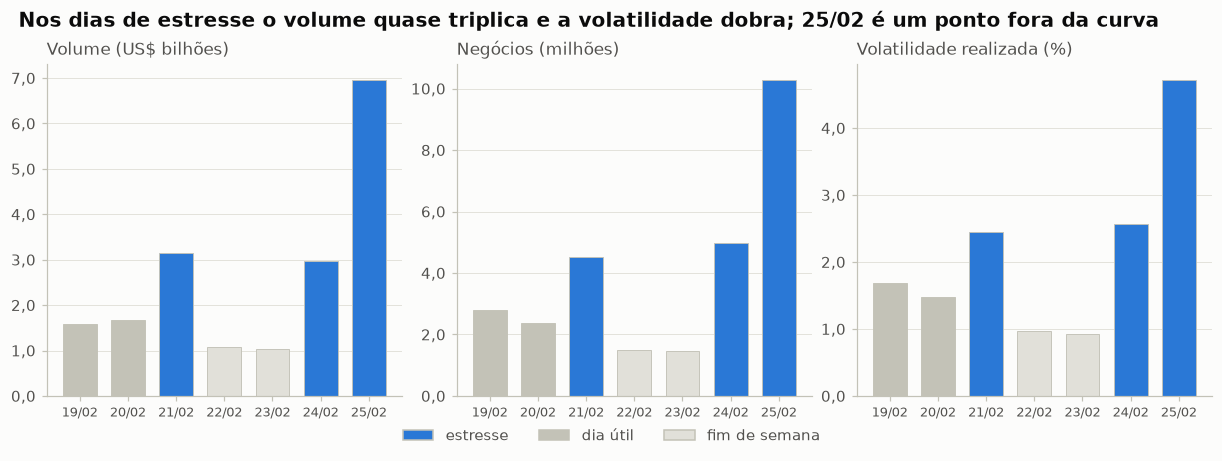
\includegraphics[width=\textwidth]{figuras/fig_resumo_diario.png}
\end{center}
\fontedados
\end{figure}

A \autoref{tab:regimes} compara as médias por tipo de dia. Nos dias de estresse
(21, 24 e 25/02), o volume foi \textbf{2,7 vezes} o de um dia útil normal, o
número de negócios 2,6 vezes e a volatilidade realizada \textbf{2,0 vezes}. O dia
25/02 é um ponto fora da curva: sozinho teve 10,3 milhões de negócios, cerca de
4 vezes um dia útil normal, e \usd~7 bilhões negociados
(\autoref{fig:diario}).

\begin{table}[htbp]
\caption{\label{tab:regimes}Médias diárias por tipo de dia e razão entre estresse e dia útil}
\begin{corpotabela}
\begin{tabular}{lrrrr}
\toprule
Tipo de dia & Volume (\usd~bi) & Negócios & VR (\%) & Amplitude (\%) \\
\midrule
Dia útil (19 e 20/02) & 1,62 & 2.585.599 & 1,59 & 2,17 \\
Fim de semana (22 e 23/02) & 1,07 & 1.481.893 & 0,95 & 1,38 \\
Estresse (21, 24 e 25/02) & 4,36 & 6.596.785 & 3,24 & 6,01 \\
\midrule
Razão estresse $\div$ dia útil & 2,69 & 2,55 & 2,04 & 2,76 \\
\bottomrule
\end{tabular}
\end{corpotabela}
\fontedados
\end{table}

O perfil de tamanho também muda. O agrupamento em dois níveis (tipo de dia
$\times$ faixa de tamanho) sobre as ordens agressoras mostra que, em estresse, as
ordens de \usd~100 mil ou mais passam de 35,9\,\% para 40,2\,\% do volume
(\autoref{tab:mixtamanho}). A \autoref{tab:grandes} mostra que só em 25/02
foram quase 10 mil dessas ordens, cerca de 4,5 vezes a média de um dia útil
normal, com ticket mediano estável perto de \usd~180 mil: o que cresce em
estresse é a quantidade de ordens institucionais, não o seu tamanho típico.

\begin{table}[htbp]
\caption{\label{tab:mixtamanho}Participação de cada faixa de tamanho no volume das ordens agressoras, por tipo de dia (\%)}
\begin{corpotabela}
\begin{tabular}{lrrrrr}
\toprule
Tipo de dia & $<$ \usd~100 & \usd~100 a 1 mil & \usd~1 a 10 mil & \usd~10 a 100 mil & $\geq$ \usd~100 mil \\
\midrule
Dia útil & 0,5 & 2,5 & 18,1 & 43,0 & 35,9 \\
Fim de semana & 0,6 & 3,6 & 17,2 & 40,8 & 37,9 \\
Estresse & 0,3 & 2,4 & 15,1 & 41,9 & 40,2 \\
\bottomrule
\end{tabular}
\end{corpotabela}
\fontedados
\end{table}

\begin{table}[htbp]
\caption{\label{tab:grandes}Ordens agressoras de \usd~100 mil ou mais, por dia}
\begin{corpotabela}
\begin{tabular}{lrrrr}
\toprule
Dia & Ordens & Volume (\usd~mi) & Ticket mediano (\usd~mil) & Maior ordem (\usd~mi) \\
\midrule
qua 19/02 & 2.066 & 531,8 & 177,8 & 3,1 \\
qui 20/02 & 2.346 & 631,6 & 187,6 & 5,1 \\
sex 21/02 & 5.100 & 1.367,0 & 185,0 & 3,4 \\
sáb 22/02 & 1.514 & 469,1 & 197,2 & 7,2 \\
dom 23/02 & 1.098 & 338,8 & 191,9 & 4,8 \\
seg 24/02 & 4.675 & 1.200,9 & 176,4 & 5,4 \\
ter 25/02 & 9.897 & 2.694,2 & 176,1 & 5,4 \\
\bottomrule
\end{tabular}
\end{corpotabela}
\fontedados
\end{table}

\section{Perfil intradiário da liquidez}\label{sec:intradiario}

Para a pergunta P1, usou-se a \textbf{mediana} por hora do dia: com apenas sete
dias, a média seria puxada pelos picos de 24 e 25/02. A
\autoref{fig:perfilhorario} mostra o volume, o número de negócios e a amplitude
medianos por minuto em cada hora UTC (no horário de Brasília, subtraem-se
3 horas).

\begin{figure}[htbp]
\caption{\label{fig:perfilhorario}Perfil horário de volume, negócios e amplitude por minuto (medianas, UTC)}
\begin{center}
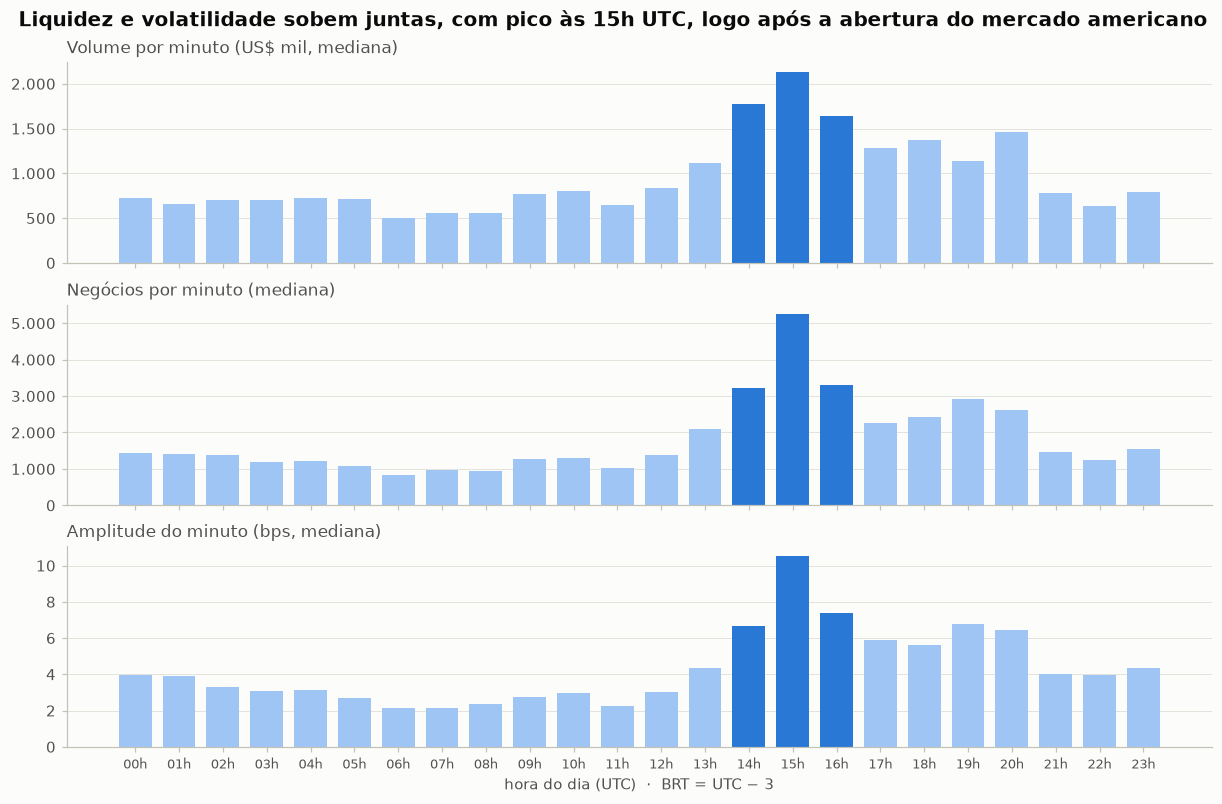
\includegraphics[width=\textwidth]{figuras/fig_perfil_horario.png}
\end{center}
\fontedados
\end{figure}

A liquidez é fortemente concentrada logo após a abertura do mercado americano,
entre 14h e 16h~UTC (11h e 13h em Brasília). Às 15h~UTC o volume mediano é de
\usd~2,13 milhões por minuto, \textbf{4,2 vezes} o das 06h~UTC (\usd~0,51 milhão
por minuto), a hora mais fraca. A volatilidade sobe junto: a correlação de
Spearman entre volume e amplitude é de $\rho = 0,83$ entre as 24 horas e de
$\rho = 0,79$ minuto a minuto. O mapa de calor da \autoref{fig:heatmap} revela,
porém, que a hora de maior volume da semana foi às 07h~UTC de 25/02, durante o
pânico: em estresse, a liquidez aparece fora do horário habitual.

\begin{figure}[htbp]
\caption{\label{fig:heatmap}Volume negociado por dia e hora (\usd~milhões por hora, UTC)}
\begin{center}
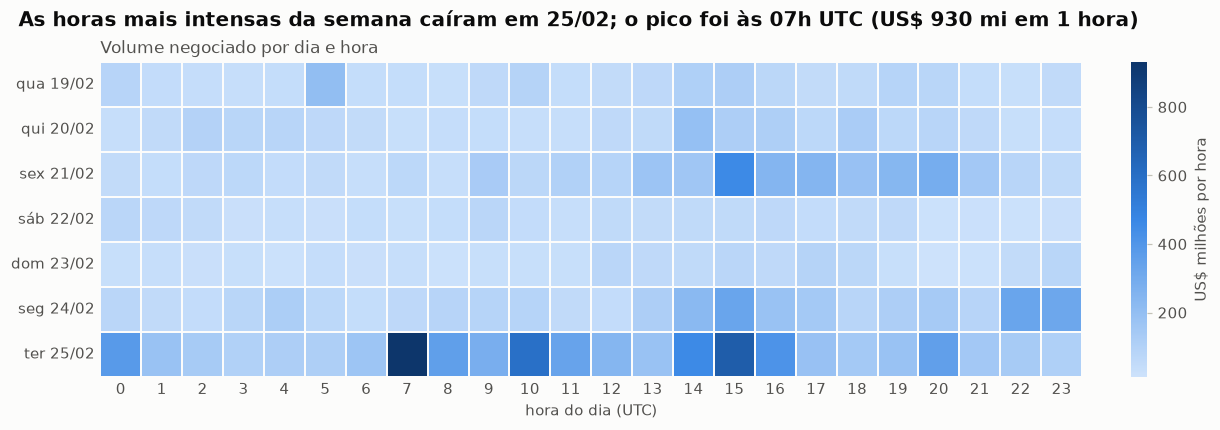
\includegraphics[width=\textwidth]{figuras/fig_heatmap_volume.png}
\end{center}
\fontedados
\end{figure}

\section{Retornos e caudas pesadas}\label{sec:caudas}

Os retornos de 1 minuto têm desvio-padrão $\sigma = 6,4$~bps e curtose em excesso
de 14,5. A \autoref{fig:caudas} compara o histograma observado, em escala
logarítmica, com uma distribuição normal de mesma média e desvio. Movimentos
além de $3\sigma$ ocorrem em \textbf{1,87\,\%} dos minutos, contra 0,27\,\% previstos
pela normal, ou seja, \textbf{6,9 vezes} mais, o que confirma as caudas pesadas
descritas por \citeonline{cont2001}. Para a mesa, limites de risco calibrados
pela curva normal subestimam a frequência de choques.

\begin{figure}[htbp]
\caption{\label{fig:caudas}Distribuição dos retornos de 1 minuto comparada à normal}
\begin{center}
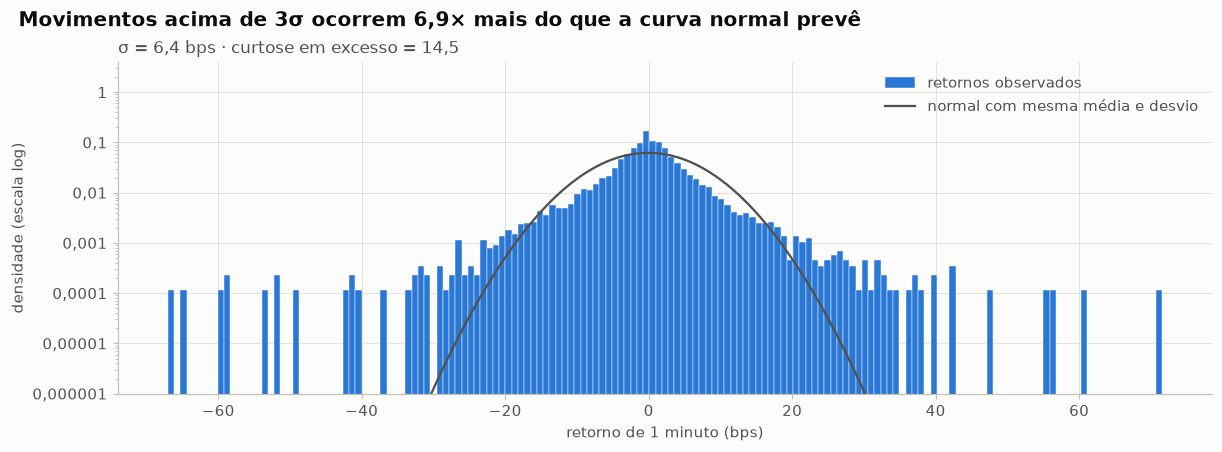
\includegraphics[width=\textwidth]{figuras/fig_caudas_retornos.png}
\end{center}
\fontedados
\end{figure}

\section{Pressão compradora e vendedora}\label{sec:pressao}

O saldo de fluxo agressor foi \textbf{negativo em todos os sete dias}, com mais
venda agressora que compra (de $-2,0\,\%$ em 20/02 a $-15,1\,\%$ em 23/02),
coerente com a queda de 13,5\,\% na semana. O painel direito da
\autoref{fig:ofi} mostra que, minuto a minuto, o OFI e o retorno do
\textbf{mesmo} minuto andam juntos.

\begin{figure}[htbp]
\caption{\label{fig:ofi}Saldo de fluxo diário e relação entre OFI e retorno no mesmo minuto}
\begin{center}
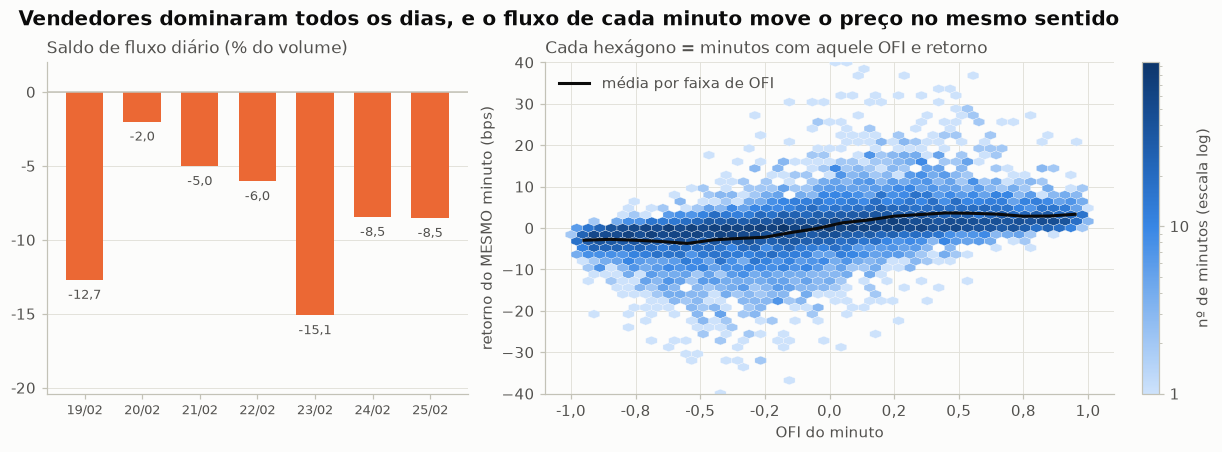
\includegraphics[width=\textwidth]{figuras/fig_ofi_fluxo.png}
\end{center}
\fontedados
\end{figure}

A pergunta P3, porém, é se o OFI \textbf{antecipa} o preço. A
\autoref{tab:defasagens} e a \autoref{fig:defasagens} mostram a correlação entre
o OFI do minuto $t$ e o retorno do minuto $t+k$. A faixa de ruído de 95\,\% para
$n = 10.080$ é $\pm 1,96/\sqrt{n} \approx \pm 0,0195$.

\begin{table}[htbp]
\caption{\label{tab:defasagens}Correlação entre $\mathrm{OFI}_t$ e $r_{t+k}$ para defasagens de 0 a 10 minutos}
\begin{corpotabela}
\setlength{\tabcolsep}{4.2pt}
\begin{tabular}{lrrrrrrrrrrr}
\toprule
$k$ (min) & 0 & 1 & 2 & 3 & 4 & 5 & 6 & 7 & 8 & 9 & 10 \\
\midrule
Pearson & 0,388 & 0,022 & 0,003 & $-0,017$ & $-0,008$ & $-0,016$ & $-0,010$ & $-0,005$ & $-0,007$ & 0,001 & $-0,010$ \\
Spearman & 0,545 & 0,038 & $-0,005$ & $-0,028$ & $-0,017$ & $-0,009$ & $-0,012$ & $-0,005$ & $-0,010$ & $-0,006$ & $-0,022$ \\
\bottomrule
\end{tabular}
\end{corpotabela}
\fontedados
\end{table}

\begin{figure}[htbp]
\caption{\label{fig:defasagens}Correlação de Pearson entre o OFI do minuto $t$ e o retorno do minuto $t+k$}
\begin{center}
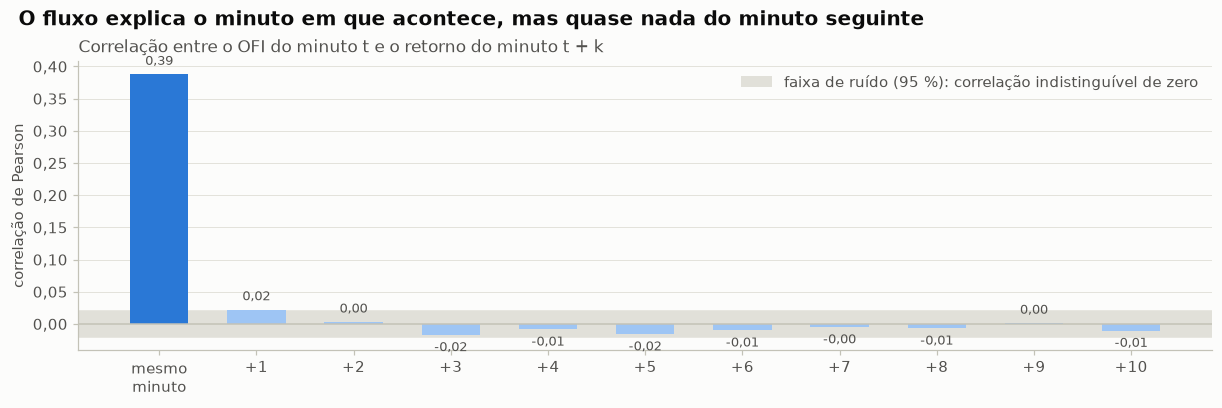
\includegraphics[width=\textwidth]{figuras/fig_ofi_defasagens.png}
\end{center}
\fontedados
\end{figure}

No mesmo minuto, a correlação de Pearson é de 0,388 (Spearman de 0,545): o fluxo
agressor empurra o preço no instante da execução. No minuto seguinte, cai para
0,022, pouco acima da faixa de ruído, o que explica apenas $r^2 \approx 0,05\,\%$
da variância do retorno, um valor economicamente desprezível. Da segunda
defasagem em diante, nenhum coeficiente de Pearson sai da faixa de ruído.

\section{Correlação entre as variáveis de 1 minuto}\label{sec:correlacao}

A \autoref{fig:spearman} mostra a matriz de correlação de Spearman, robusta às
caudas pesadas, entre as principais variáveis das barras de 1 minuto. Atividade
(volume e número de negócios), amplitude e retorno absoluto formam um bloco
fortemente correlacionado ($\rho$ entre 0,58 e 0,92). O OFI praticamente não se
relaciona com essas medidas de intensidade e só se liga ao retorno com sinal
($\rho = 0,55$). Essa separação antecipa o resultado do
\autoref{cap:modelagem}: a volatilidade é previsível a partir da atividade
recente, mas a direção não.

\begin{figure}[htbp]
\caption{\label{fig:spearman}Matriz de correlação de Spearman entre as variáveis de 1 minuto}
\begin{center}
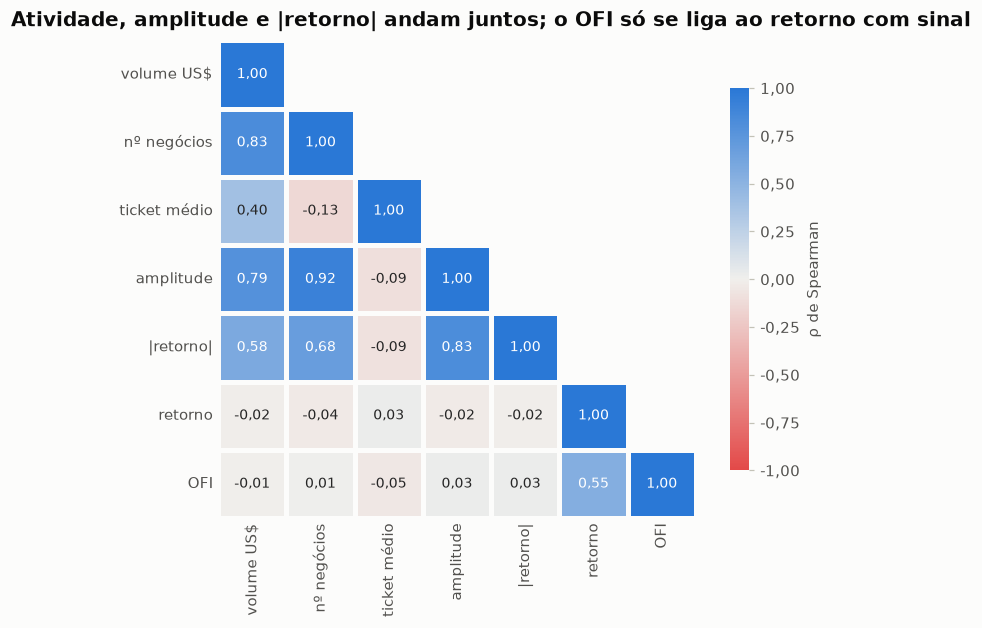
\includegraphics[width=0.78\textwidth]{figuras/fig_correlacao_spearman.png}
\end{center}
\fontedados
\end{figure}

\section{Respostas às perguntas de negócio}\label{sec:respostas}

A \autoref{tab:kpis} consolida os indicadores que respondem às três perguntas.

\begin{table}[htbp]
\caption{\label{tab:kpis}Indicadores-chave que respondem às perguntas P1 a P3}
\begin{corpotabela}
\begin{tabular}{llr}
\toprule
Pergunta & Indicador & Valor \\
\midrule
P1 & Hora de maior volume (mediana por minuto) & 15h UTC (\usd~2,13 mi/min) \\
P1 & Hora de menor volume (mediana por minuto) & 06h UTC (\usd~0,51 mi/min) \\
P1 & Razão entre pico e vale & 4,2 \\
P1 & Spearman entre volume e amplitude (24 horas) & 0,83 \\
P2 & Volume médio em estresse $\div$ dia útil & 2,7 \\
P2 & Volatilidade realizada em estresse $\div$ dia útil & 2,0 \\
P2 & Participação no volume dos negócios $\geq$ \usd~10 mil & 59,8\,\% \\
P2 & Participação na contagem dos negócios $\geq$ \usd~10 mil & 1,42\,\% \\
P3 & Correlação entre OFI e retorno no mesmo minuto & 0,388 \\
P3 & Correlação entre OFI e retorno do minuto seguinte & 0,022 \\
P3 & Dias com mais venda que compra agressora & 7 de 7 \\
\bottomrule
\end{tabular}
\end{corpotabela}
\fontedados
\end{table}

\textbf{P1 -- Liquidez e janela de execução.} A liquidez concentra-se entre 14h e
16h~UTC, com pico às 15h~UTC, e a volatilidade sobe junto. Para a mesa, isso é um
\textit{trade-off}: o horário mais líquido absorve ordens grandes com menos
impacto, mas expõe a execução a movimentos mais bruscos. A recomendação é fatiar
ordens grandes (TWAP ou VWAP) dentro da janela de liquidez, sem executar tudo de
uma vez nos minutos de pico de volatilidade, e monitorar deslocamentos da
liquidez em dias de choque.

\textbf{P2 -- Dias de estresse.} Pela regra objetiva, 21, 24 e 25/02 foram dias de
estresse, com volume 2,7 vezes e volatilidade 2,0 vezes maiores que um dia útil
normal. O volume é concentrado em poucos negócios grandes, e essa concentração
aumenta em estresse. Limites de risco e alertas devem ser calibrados pela
volatilidade realizada, e a infraestrutura deve suportar cerca de 4 vezes a carga
de um dia útil.

\textbf{P3 -- Fluxo de ordens.} O fluxo explica o retorno do minuto em que ocorre,
mas quase nada do minuto seguinte. De forma isolada e linear, o OFI de 1 minuto
não antecipa o preço de maneira útil, o que é consistente com um mercado
eficiente nessa escala \cite{fama1970}. O \autoref{cap:modelagem} testa essa
conclusão com horizontes mais curtos, combinações de variáveis e modelos não
lineares.
